\section{Discussion}
\label{sec:discussion}
The process of getting our results provided insight into the redundancies that exist within mobile web pages. We first observed that pages that are designed for mobile browsers are only a fraction of the size of pages designed for desktop browsers. In addition to size, we also know that the way that mobile sites are structured are inherently different through observation. This shows that it is worth exploring the types of redundancies that exist within mobile sites. This information can be used in the future to examine how these redundancies are similar to or different from desktop browser site redundancies. It can also be used to design caches that will take advantage of the redundancy patterns that we find. 

As for chunk size, we found that a chunk size close to 10 bytes was optimal in the trade-off between obtaining a low miss-rate and reducing the number of bytes of fingerprints transferred back and forth between the proxy and mobile device. Based on the feedback we received after our presentation, we also began implementing the sliding window chunking methodology so that we would not be constrained to a fixed chunk size and so that we would find a larger percentage of deduplicated data. 

There were multiple design decisions that we considered before constructing the protocol. We designed our protocol such that fingerprint computation only occurs at the proxy. This is because mobile devices tend to have limited computational capacity and if the heavy lifting is deferred to the proxy, then the mobile device simply has to do look-ups to determine cache hits and misses. However, the drawback in this approach is that we incur the overhead of passing fingerprints across the network, leading to possible latency and additional power consumption. In addition, it also reduces the benefits of bandwidth reductions obtained by chunking.

We build a secondary protocol implementation to address the following few additional concerns. First, there is an inefficiency that comes from the additional communication that occurs between the device and proxy to send fingerprints. Second, using the MRU eviction algorithm for our tests could have possibly restricted by how much we can reduce bandwidth. To consider trade-offs in communication protocols and eviction schemes, we implemented the protocol with a url-cache as proof of concept and for testing purposes. The higher level approach is shown in Figures \ref{fig:foo} and \ref{fig:bar}. 

\begin{figure}[h] 
\centering 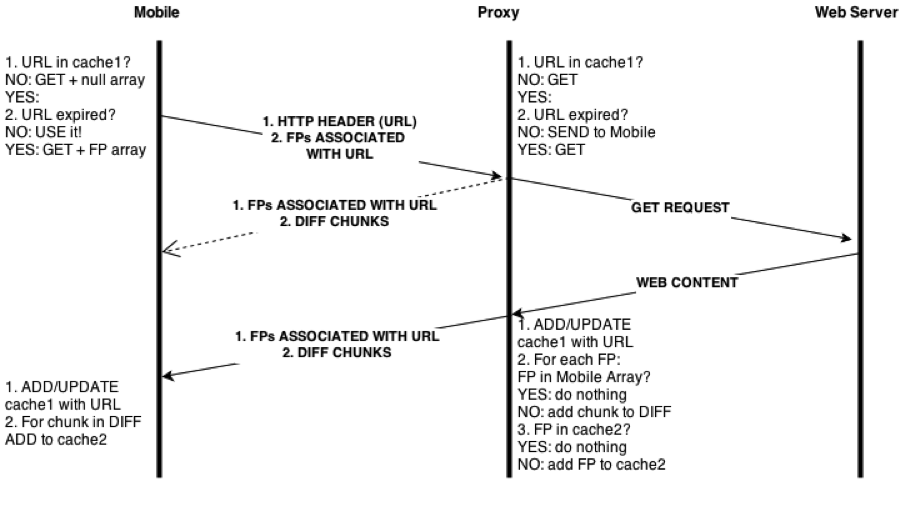
\includegraphics[width=\columnwidth]{images/urlcache-protocol.png}
\caption{Protocol. }
\label{fig:foo}
\end{figure} 
\begin{figure}[h] 
\centering 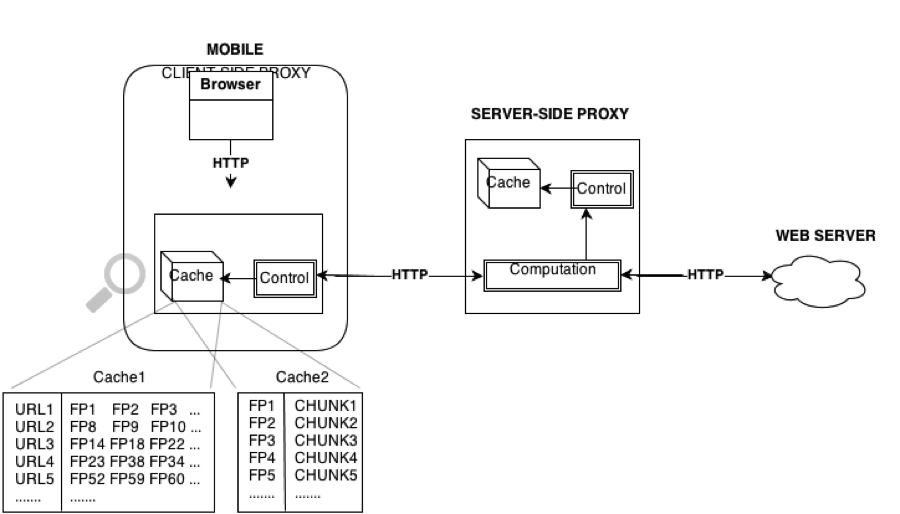
\includegraphics[width=\columnwidth]{images/url-cache-hl.png}
\caption{Url-Cache. }
\label{fig:bar}
\end{figure} 

The modified implementation works in the following way. In addition to the previous implementation we added a url-cache, shown in Figure \ref{fig:bar}, which maps each url request to the set of fingerprints that represent it. If the mobile device contains an older version, it sends the list of fingerprints to the proxy along with the requested url. The proxy then sends back the diff between the mobile's fingerprints and fingerprints of fresh content which it either obtains from its own cache or from the web server. 

Figure \ref{fig:foo} shows that it may be possible to reduce latency with this approach due to the decreased amount of communication that needs to occur between the proxy and device. In addition, preliminary testing during implementation showed that in some cases (dependent on the size of the page, whether or not an older version of it is in the cache, and pattern of 'browsing') bandwidth was reduced. The fingerprint overhead remains on the same order because the fingerprint of the entire page still needs to be sent. The bandwidth reduction for some cases came from a lower miss-rate afforded by the url-cache which was used for the eviction scheme. The Least Recently Added url was evicted from the url cache and the fingerprints that the url mapped to were evicted from the other cache as long as the fingerprint didn't overlap with the other web pages.

We also made several assumptions while implementing the protocol and testing. We assume that each time we made a request that the content in our cache was not fresh, and we did not implement a check for expiration-date or use the 'If-Modified-Since' protocol to check for freshness. We also attempted to collect data from various other websites but ran into several issues. Some websites don't have a different version for mobile devices at all. Some others had a different version, but did not use it as its response based on the User-Agent, and instead specifically required a request of the mobile url. Redirects were also not handled in the way we obtained offline data. Furthermore, we did not check to see if the data was "cacheable" and assumed that all the websites we were working with had cacheable content. Lastly, the results of our tests did not incorporate checks for content overlap between different chunks. We do however, now have an implementation of a sliding window for chunking and fingerprinting in place which is passed along the content stream to catch redundancies between different chunks that would not have been caught with fixed-sized chunks. 

A last, but minor point is the consideration of how integrity of data is affected by possible collision due to fingerprinting. We assume that we do not get collision because the size of our content is small enough that the risk of collision is negligible. 

We have thoroughly tested our implementation in various settings and with a wide range of parameter values. We have evaluated the results of chunking by using data from non-chunked protocol as control. We've done preliminary analysis on using mobile web pages by collecting offline data for desktop browsers and using it as a control. We have experimented with various chunk sizes as well as different caching algorithms. We have evaluated the effectiveness of our protocol both in terms of miss-rate as well as how that translates to the actual number of bytes transferred which gives us better insight into the amount of bandwidth that can be saved. 
